\chapter{Result}

\section{Plots of 2D data}

\subsection{Left Hippocampus, normalized and eroded}

\begin{figure}[H]
  \centering
  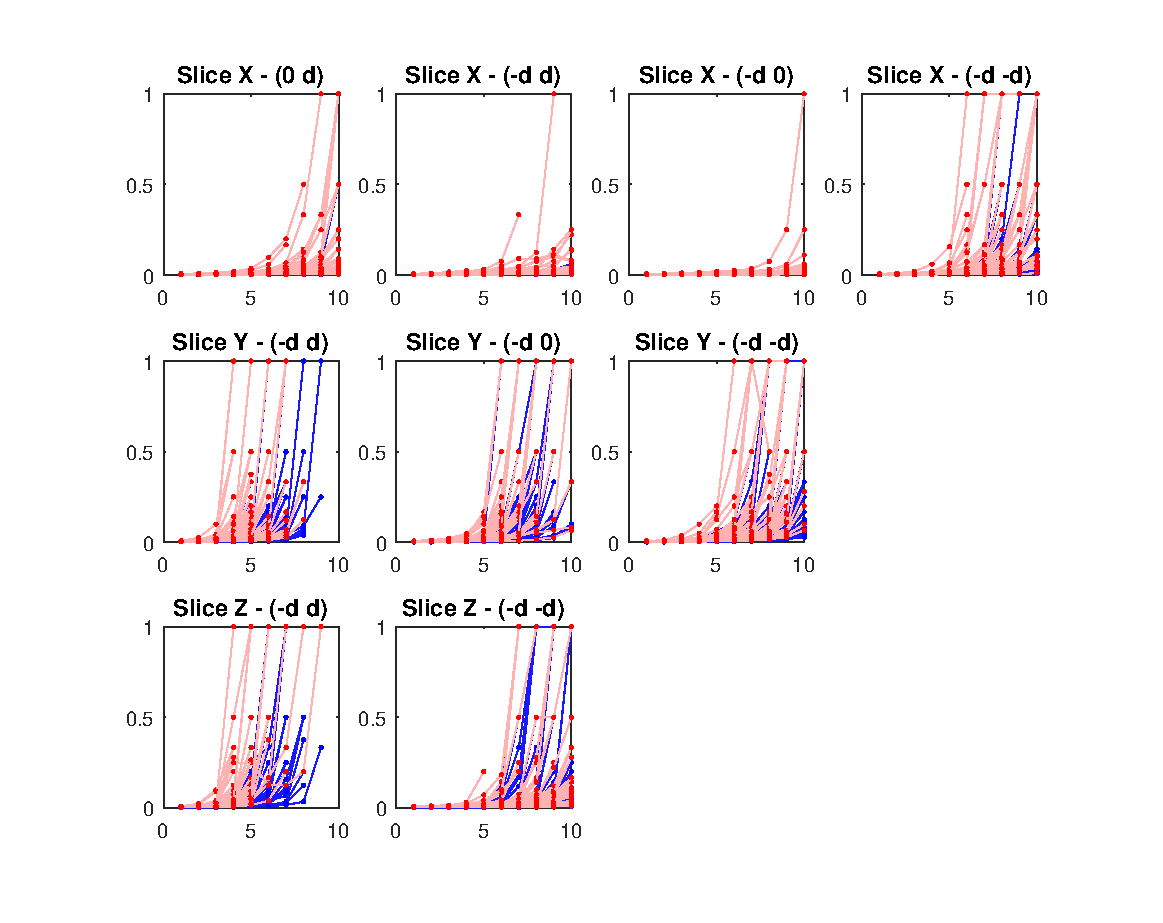
\includegraphics[scale=0.65]{ASMleftnormalizederode.eps}
  \caption{Plot of the Angular Second Moment features where the data have been normalized and eroded. The red are the patients with AD and the blue are the rest}\label{fig:ASMLeftNormalizedEroded}
\end{figure}

\begin{figure}[H]
  \centering
  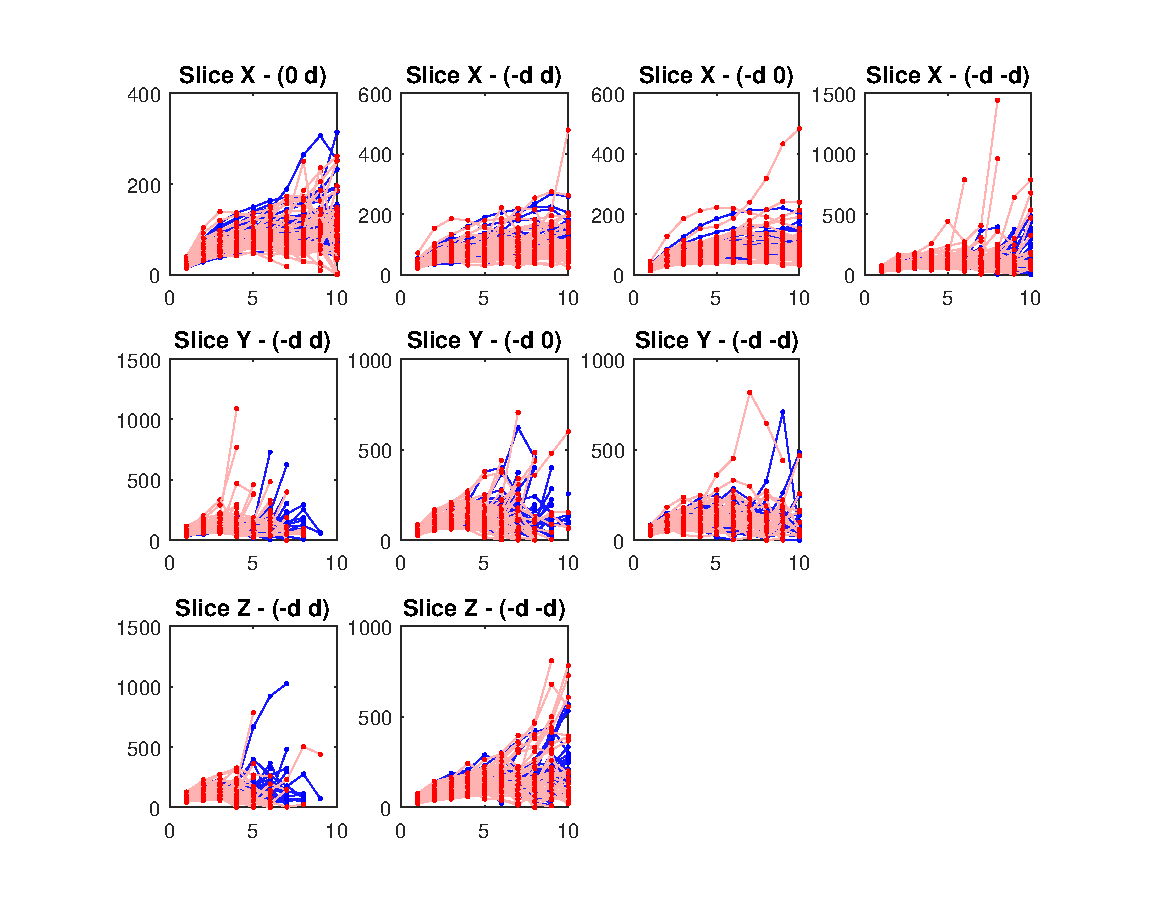
\includegraphics[scale=0.65]{Contrastleftnormalizederode.eps}
  \caption{Plot of the Contrast features where the data have been normalized and eroded. The red are the patients with AD and the blue are the rest}\label{fig:ContrastLeftNormalizedEroded}
\end{figure}

\begin{figure}[H]
  \centering
  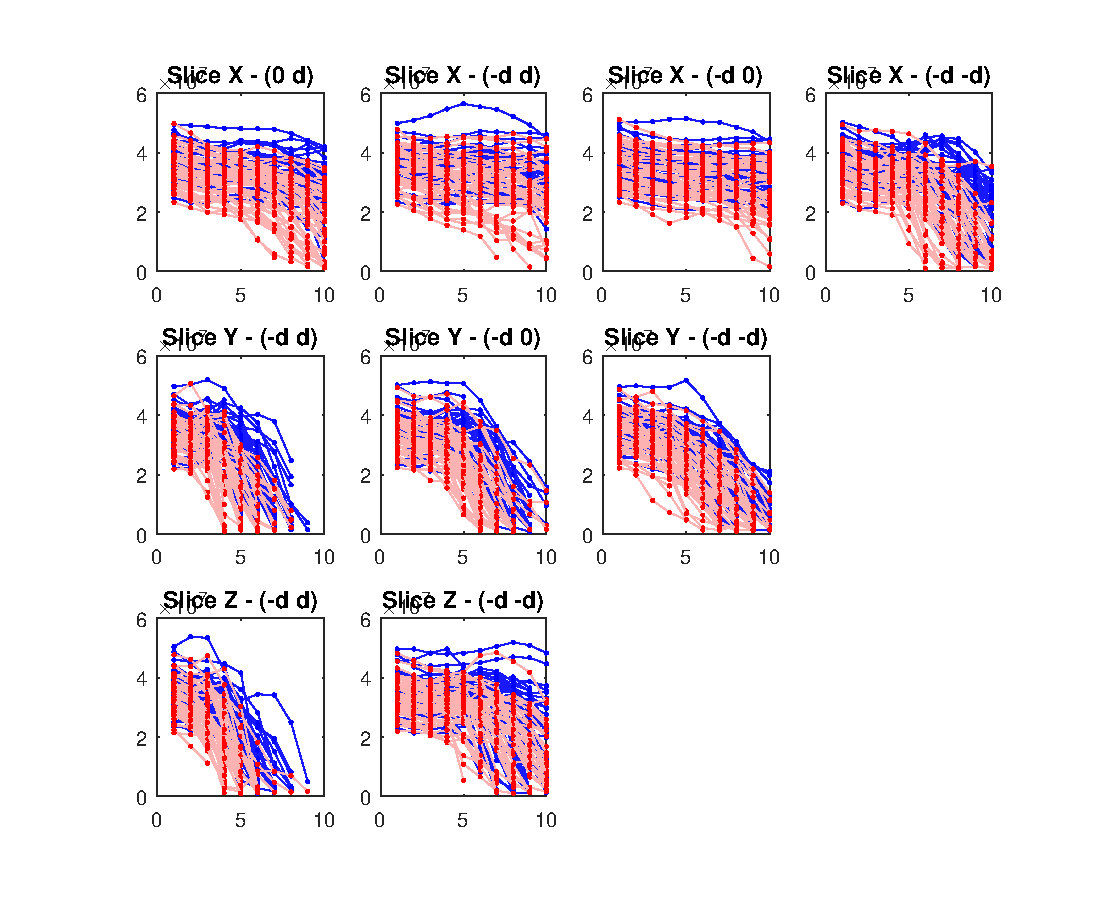
\includegraphics[scale=0.65]{Correlationleftnormalizederode.eps}
  \caption{Plot of the Correlation features where the data have been normalized and eroded. The red are the patients with AD and the blue are the rest}\label{fig:Correlationleftnormalizederode}
\end{figure}

\begin{figure}[H]
  \centering
  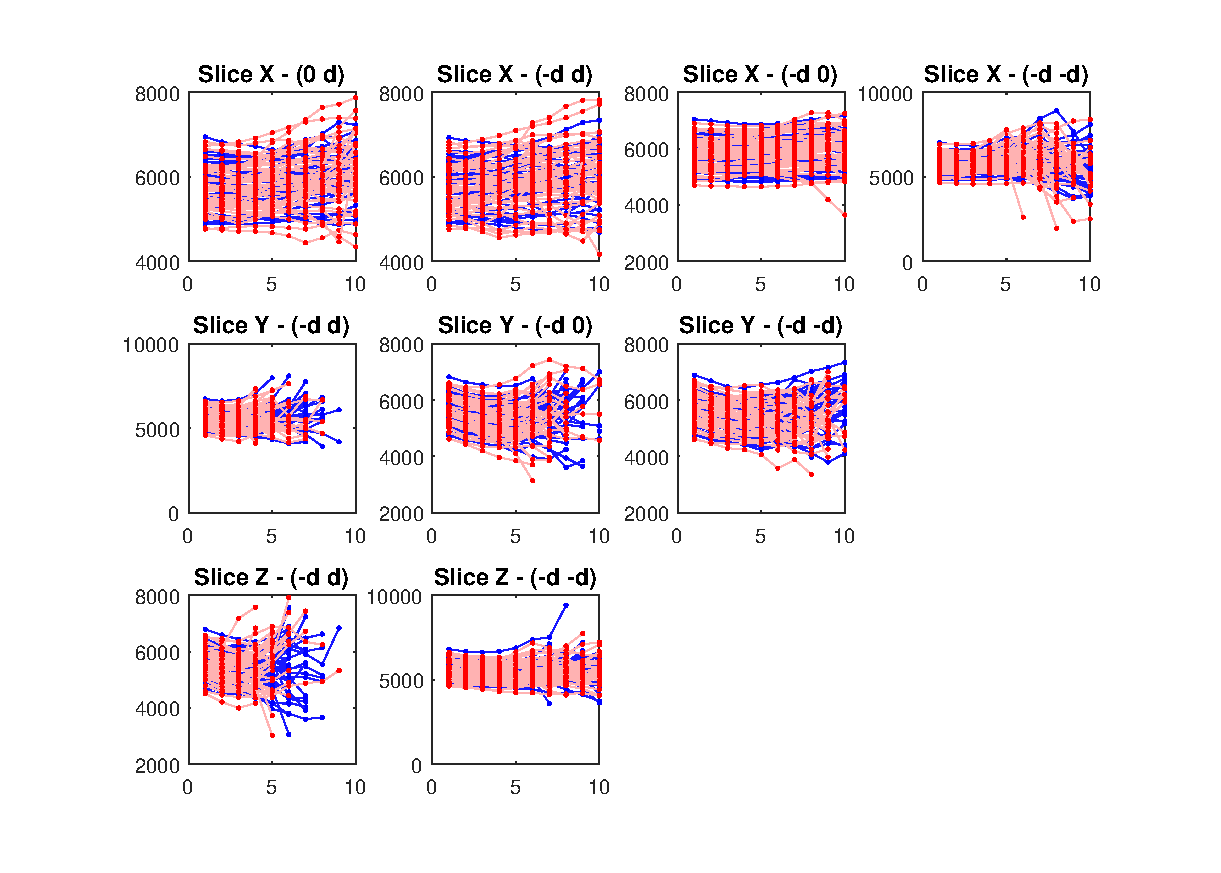
\includegraphics[scale=0.65]{Varianceleftnormalizederode.eps}
  \caption{Plot of the Variance features where the data have been normalized and eroded. The red are the patients with AD and the blue are the rest}\label{fig:Varianceleftnormalizederode}
\end{figure}

\begin{figure}[H]
  \centering
  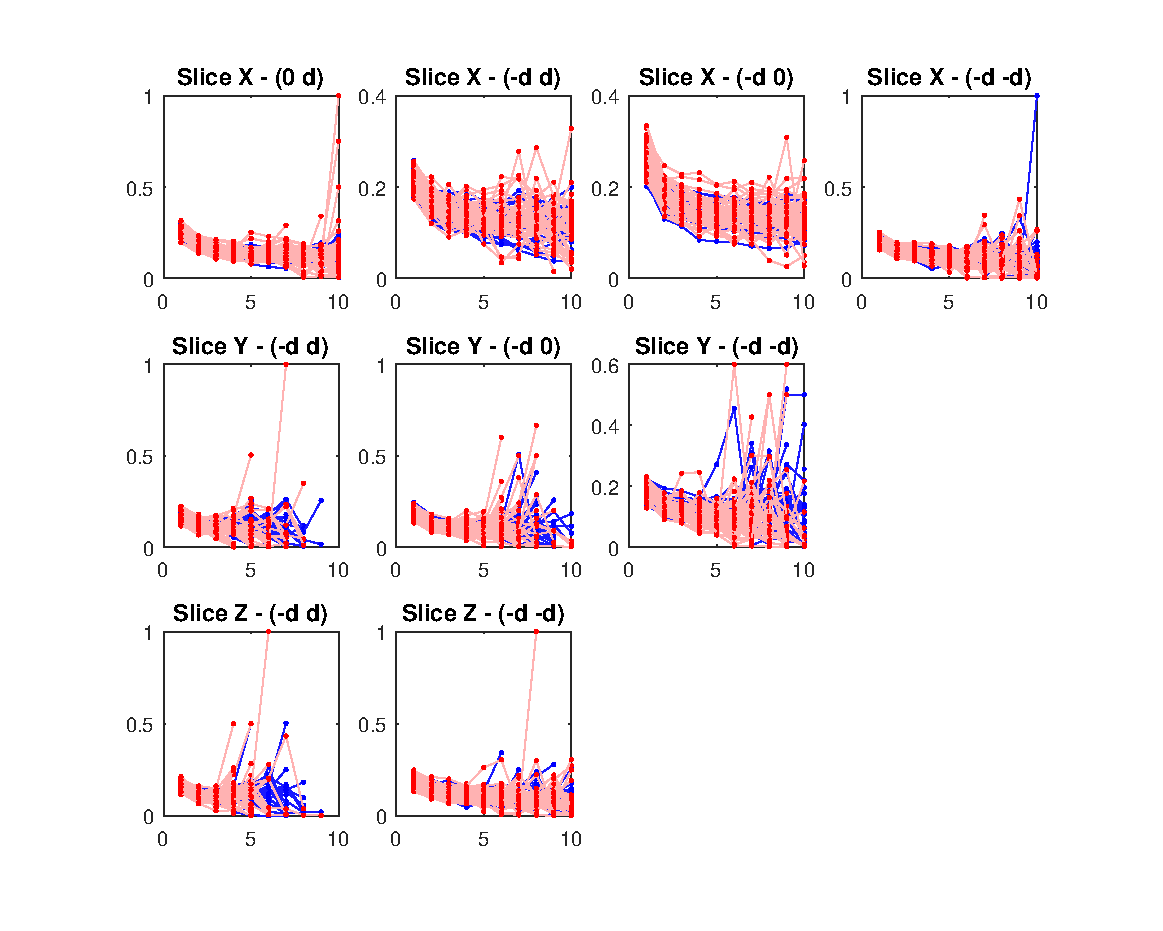
\includegraphics[scale=0.65]{IDMleftnormalizederode.eps}
  \caption{Plot of the Inverse Difference Moment features where the data have been normalized and eroded. The red are the patients with AD and the blue are the rest}\label{fig:IDMleftnormalizederode}
\end{figure}

\begin{figure}[H]
  \centering
  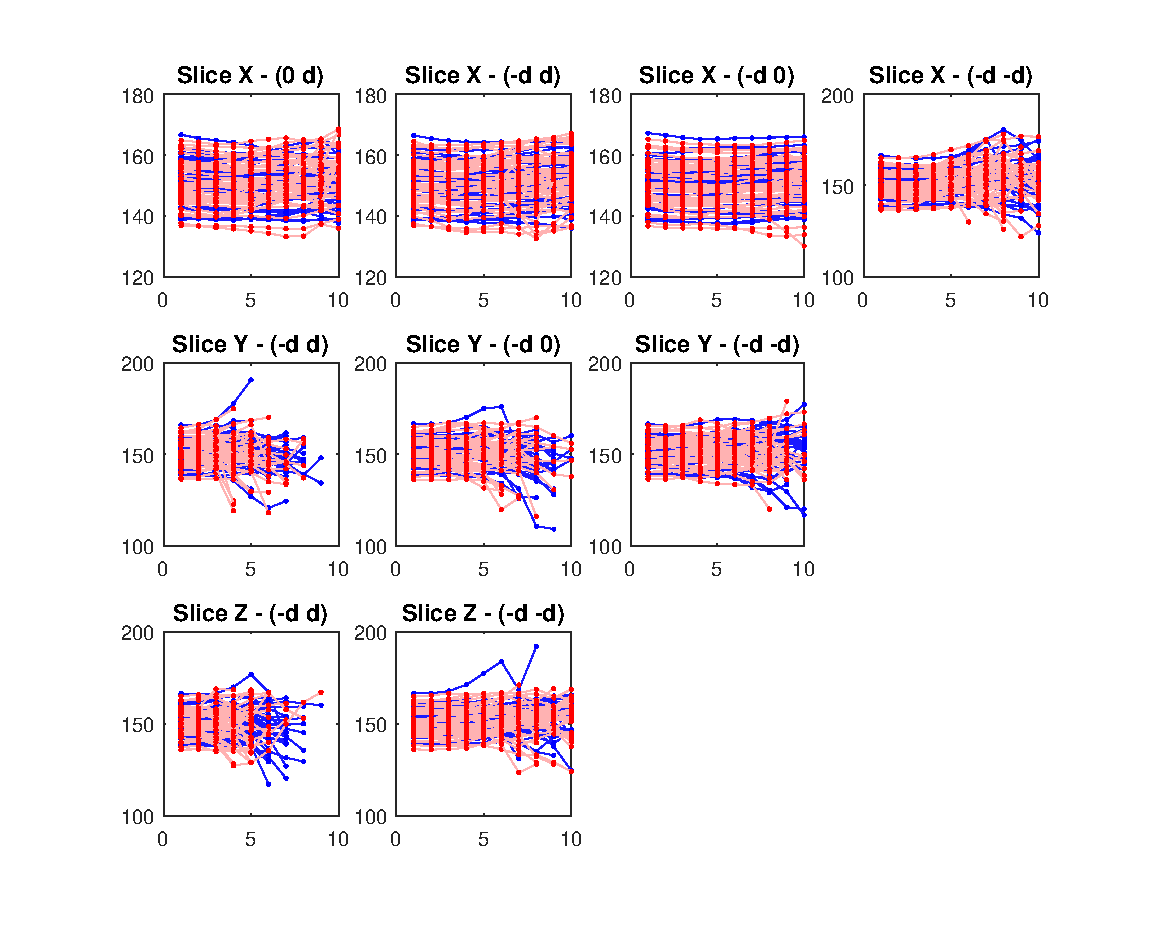
\includegraphics[scale=0.65]{SumAverageleftnormalizederode.eps}
  \caption{Plot of the Sum Average features where the data have been normalized and eroded. The red are the patients with AD and the blue are the rest}\label{fig:SumAverageleftnormalizederode}
\end{figure}

\begin{figure}[H]
  \centering
  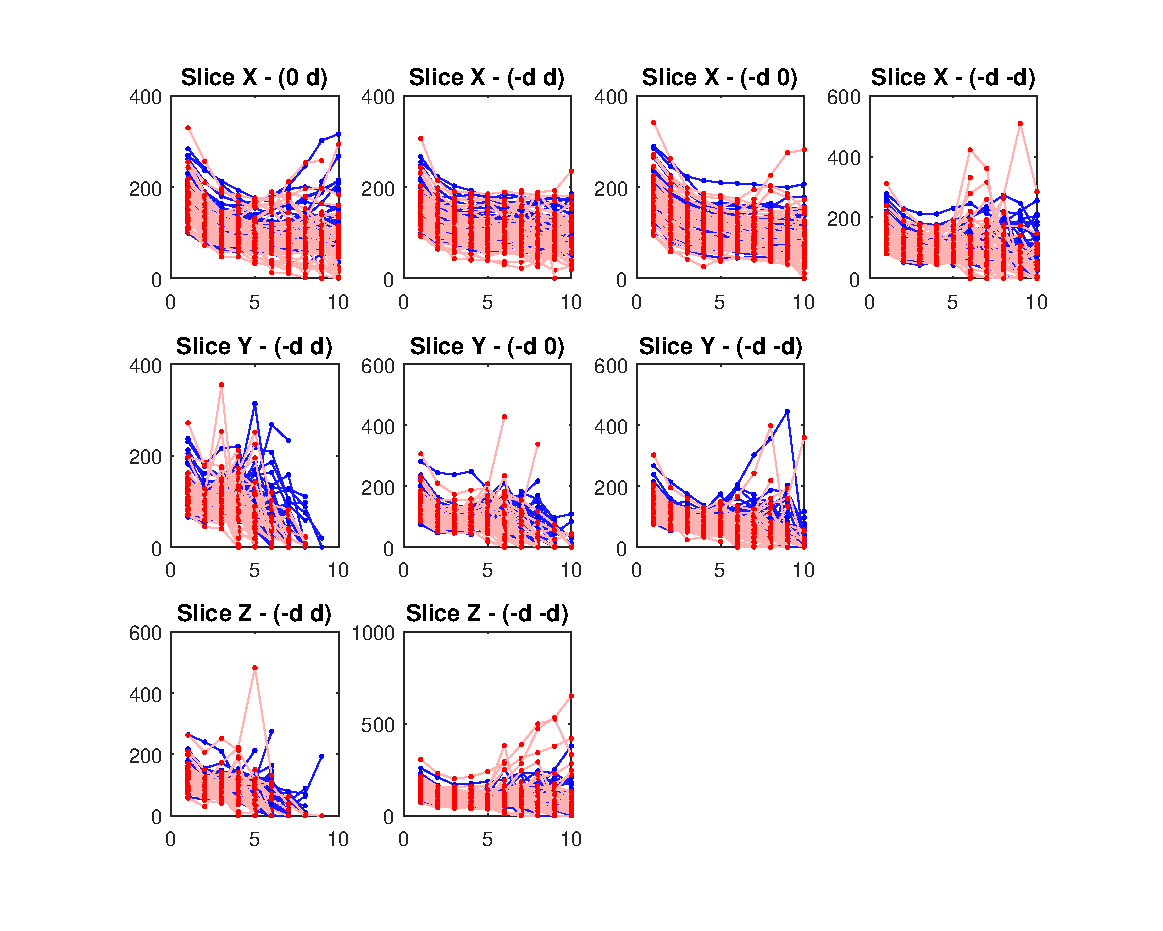
\includegraphics[scale=0.65]{SumVarianceleftnormalizederode.eps}
  \caption{Plot of the Sum Variance features where the data have been normalized and eroded. The red are the patients with AD and the blue are the rest}\label{fig:SumVarianceleftnormalizederode}
\end{figure}

\begin{figure}[H]
  \centering
  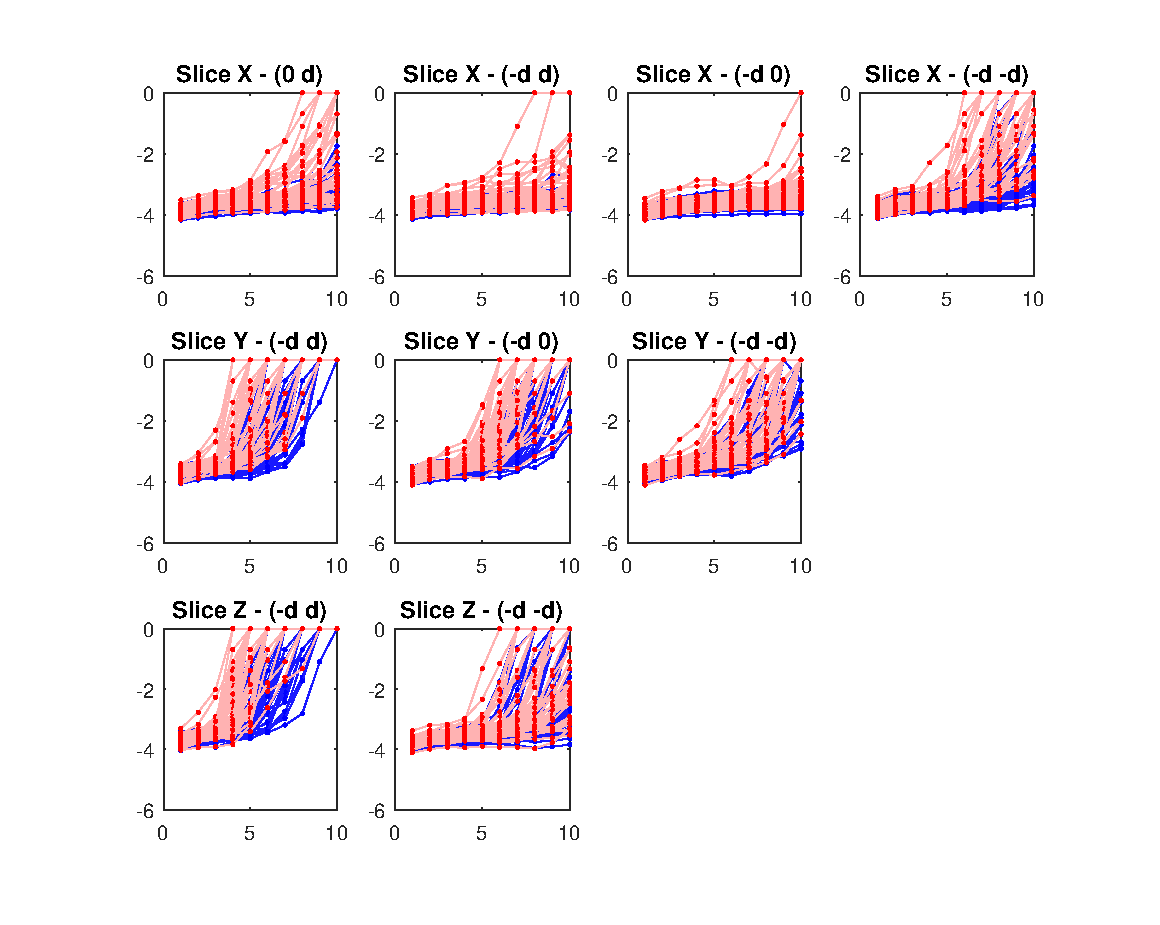
\includegraphics[scale=0.65]{SumEntropyleftnormalizederode.eps}
  \caption{Plot of the Sum Entropy features where the data have been normalized and eroded. The red are the patients with AD and the blue are the rest}\label{fig:SumEntropyleftnormalizederode}
\end{figure}

\begin{figure}[H]
  \centering
  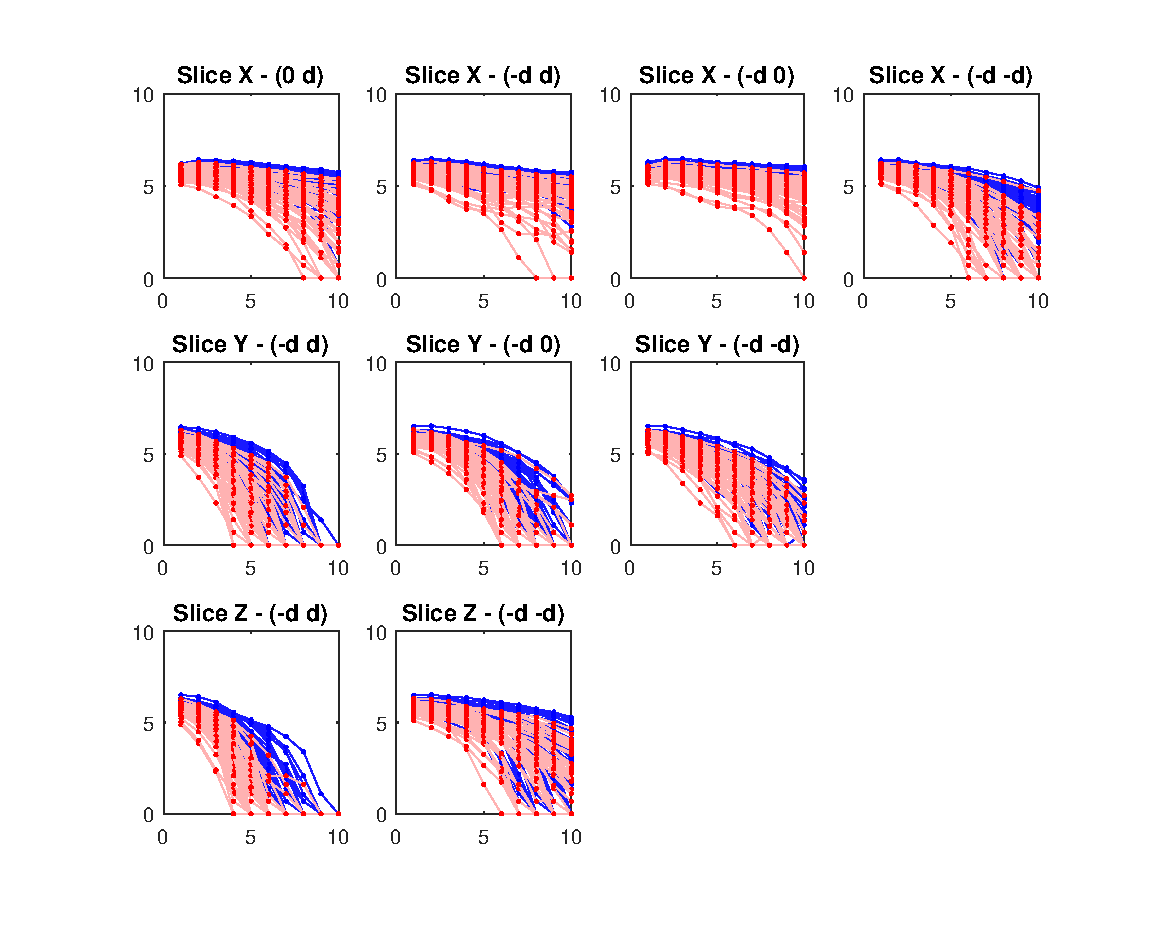
\includegraphics[scale=0.65]{Entropyleftnormalizederode.eps}
  \caption{Plot of the Entropy features where the data have been normalized and eroded. The red are the patients with AD and the blue are the rest}\label{fig:Entropyleftnormalizederode}
\end{figure}

\begin{figure}[H]
  \centering
  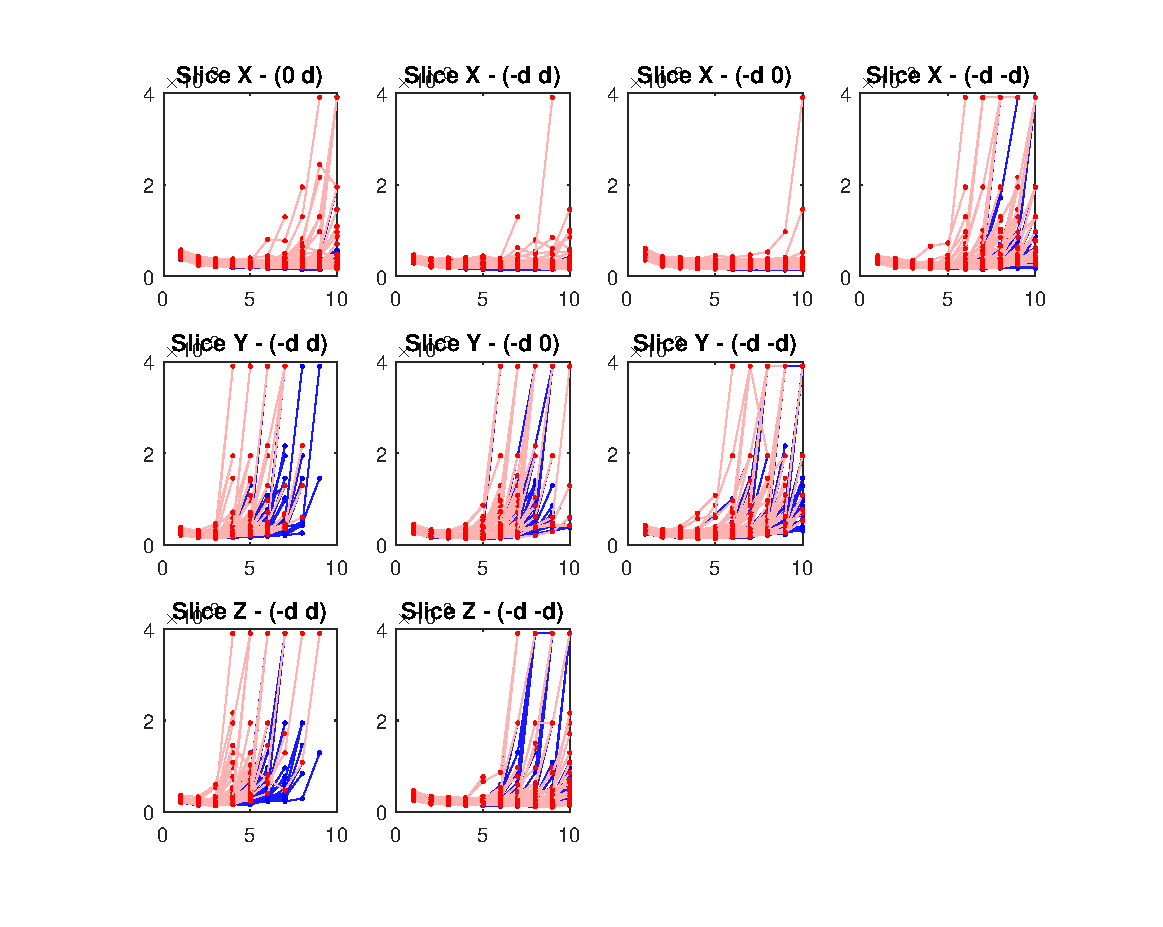
\includegraphics[scale=0.65]{DifferenceVarianceleftnormalizederode.eps}
  \caption{Plot of the Difference Variance features where the data have been normalized and eroded. The red are the patients with AD and the blue are the rest}\label{fig:DifferenceVarianceleftnormalizederode}
\end{figure}

\begin{figure}[H]
  \centering
  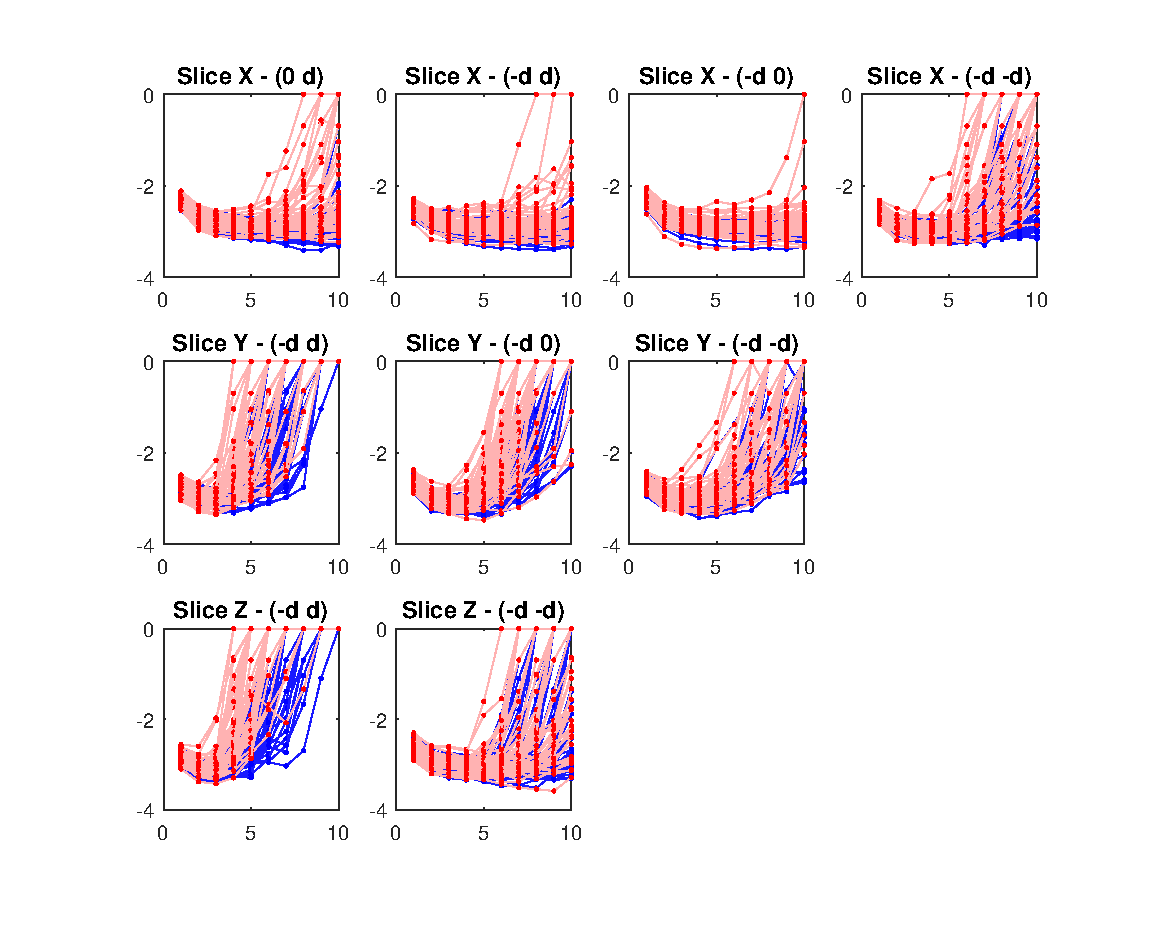
\includegraphics[scale=0.65]{DifferenceEntropyleftnormalizederode.eps}
  \caption{Plot of the Difference Entropy features where the data have been normalized and eroded. The red are the patients with AD and the blue are the rest}\label{fig:DifferenceEntropyleftnormalizederode}
\end{figure}

\begin{figure}[H]
  \centering
  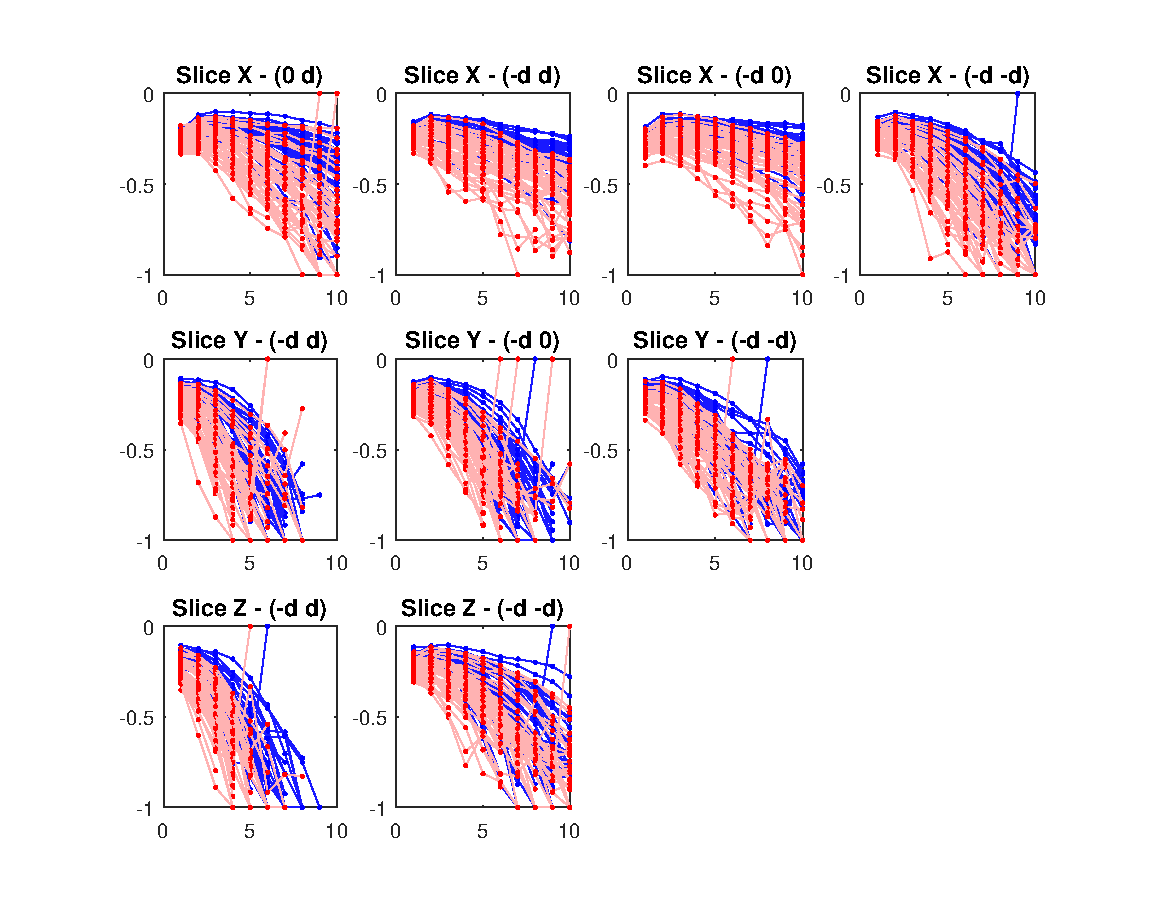
\includegraphics[scale=0.65]{IMOC1leftnormalizederode.eps}
  \caption{Plot of the Information Measures of Correlation1 features where the data have been normalized and eroded. The red are the patients with AD and the blue are the rest}\label{fig:IMOC1leftnormalizederode}
\end{figure}

\begin{figure}[H]
  \centering
  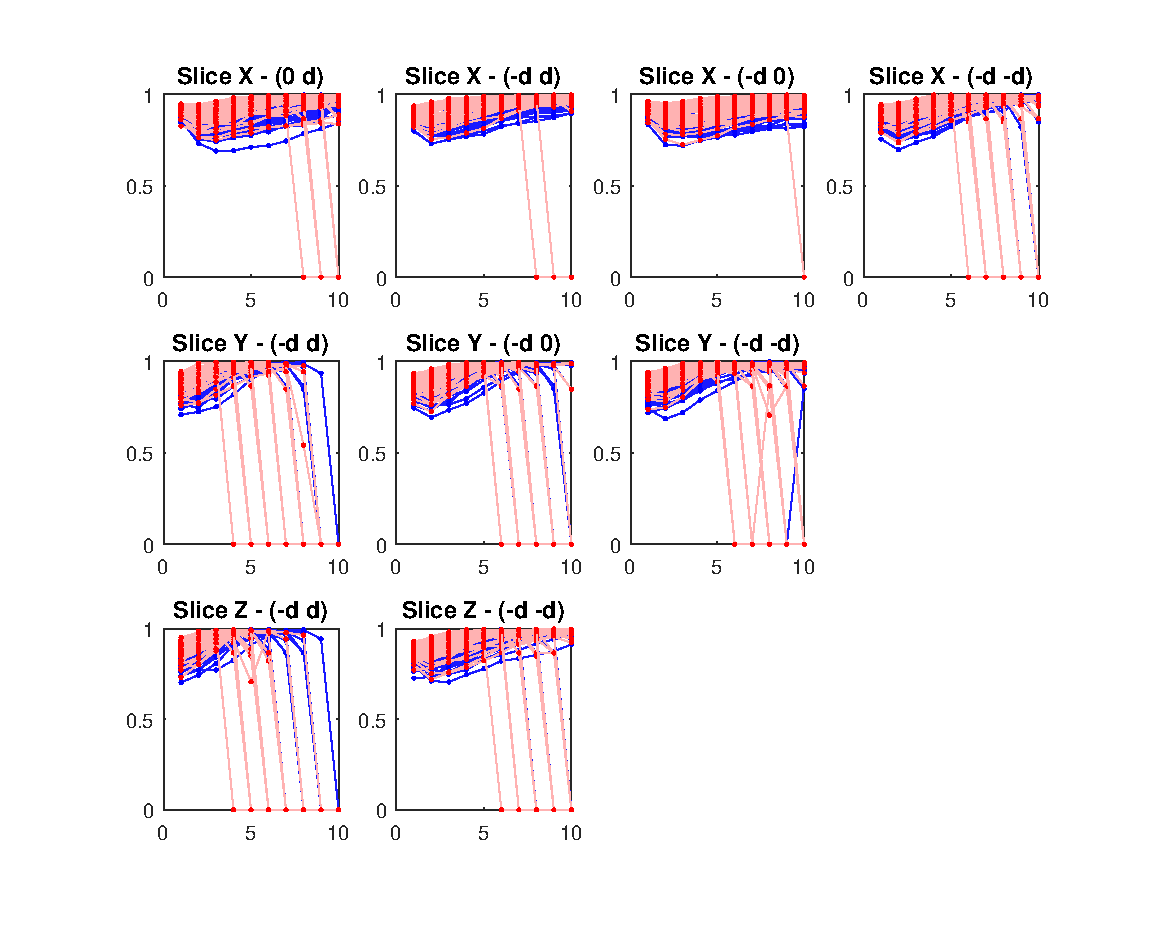
\includegraphics[scale=0.65]{IMOC2leftnormalizederode.eps}
  \caption{Plot of the Information Measures of Correlation2 features where the data have been normalized and eroded. The red are the patients with AD and the blue are the rest}\label{fig:IMOC2leftnormalizederode}
\end{figure}

\section{Plots of 3D data}

\subsection{Left Hippocampus, not normalized and eroded}

\begin{figure}[H]
  \centering
  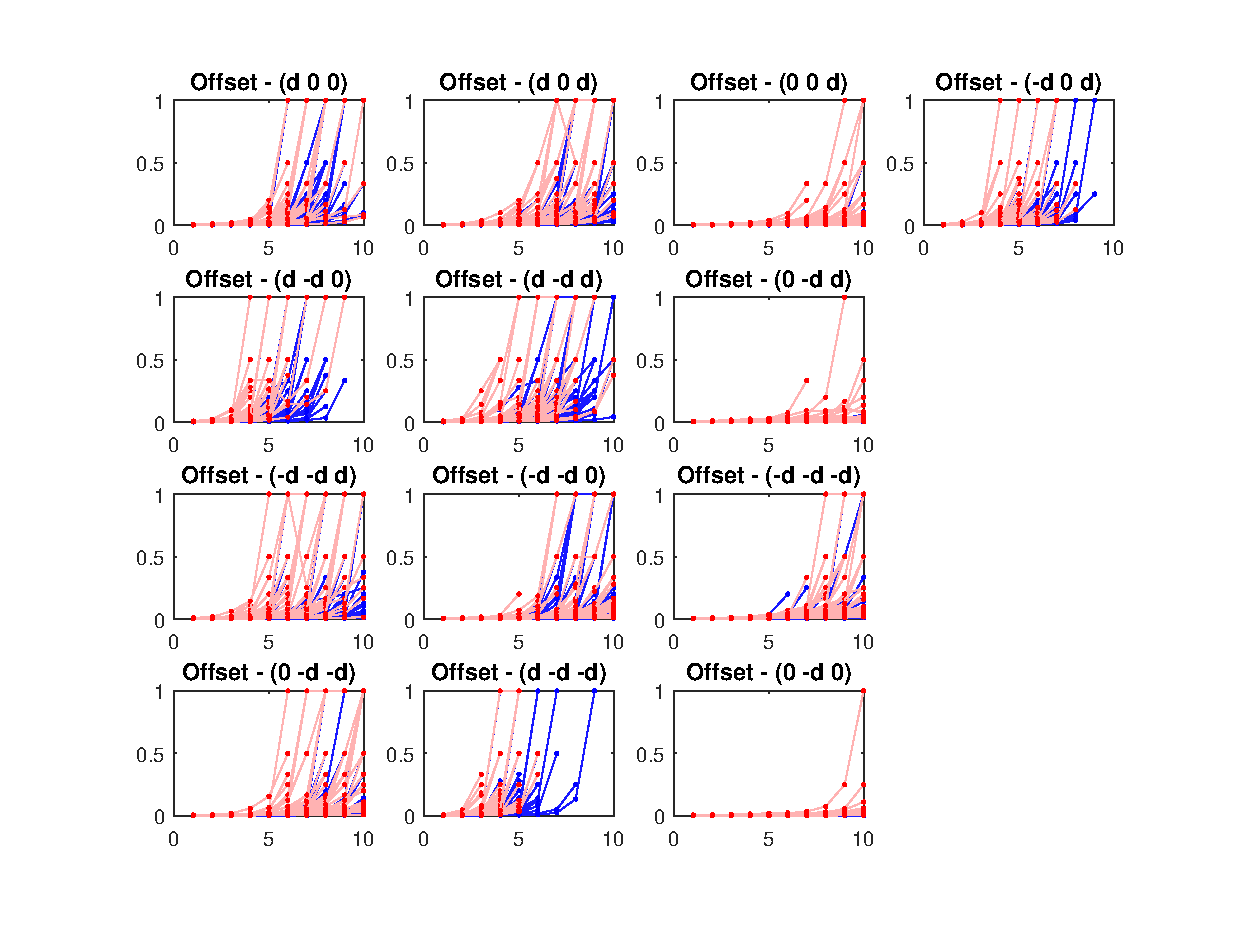
\includegraphics[scale=0.65]{ASMleftnormalizederode3D.eps}
  \caption{Plot of the Angular Second Moment features where the data have been normalized and eroded. The red are the patients with AD and the blue are the rest}\label{fig:ASMLeftNormalizedEroded3D}
\end{figure}

\begin{figure}[H]
  \centering
  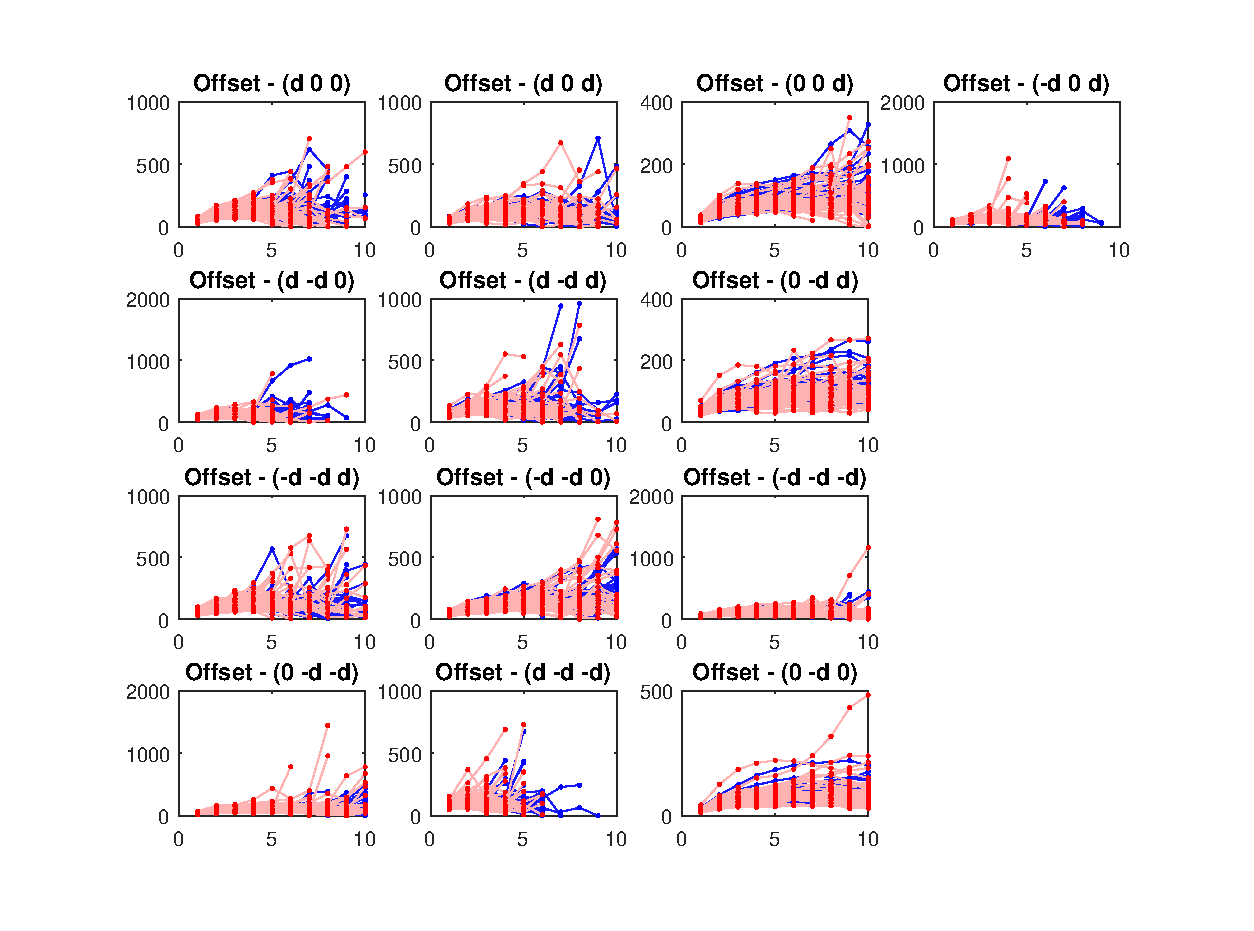
\includegraphics[scale=0.65]{Contrastleftnormalizederode3D.eps}
  \caption{Plot of the Contrast features where the data have been normalized and eroded. The red are the patients with AD and the blue are the rest}\label{fig:ContrastLeftNormalizedEroded3D}
\end{figure}

\begin{figure}[H]
  \centering
  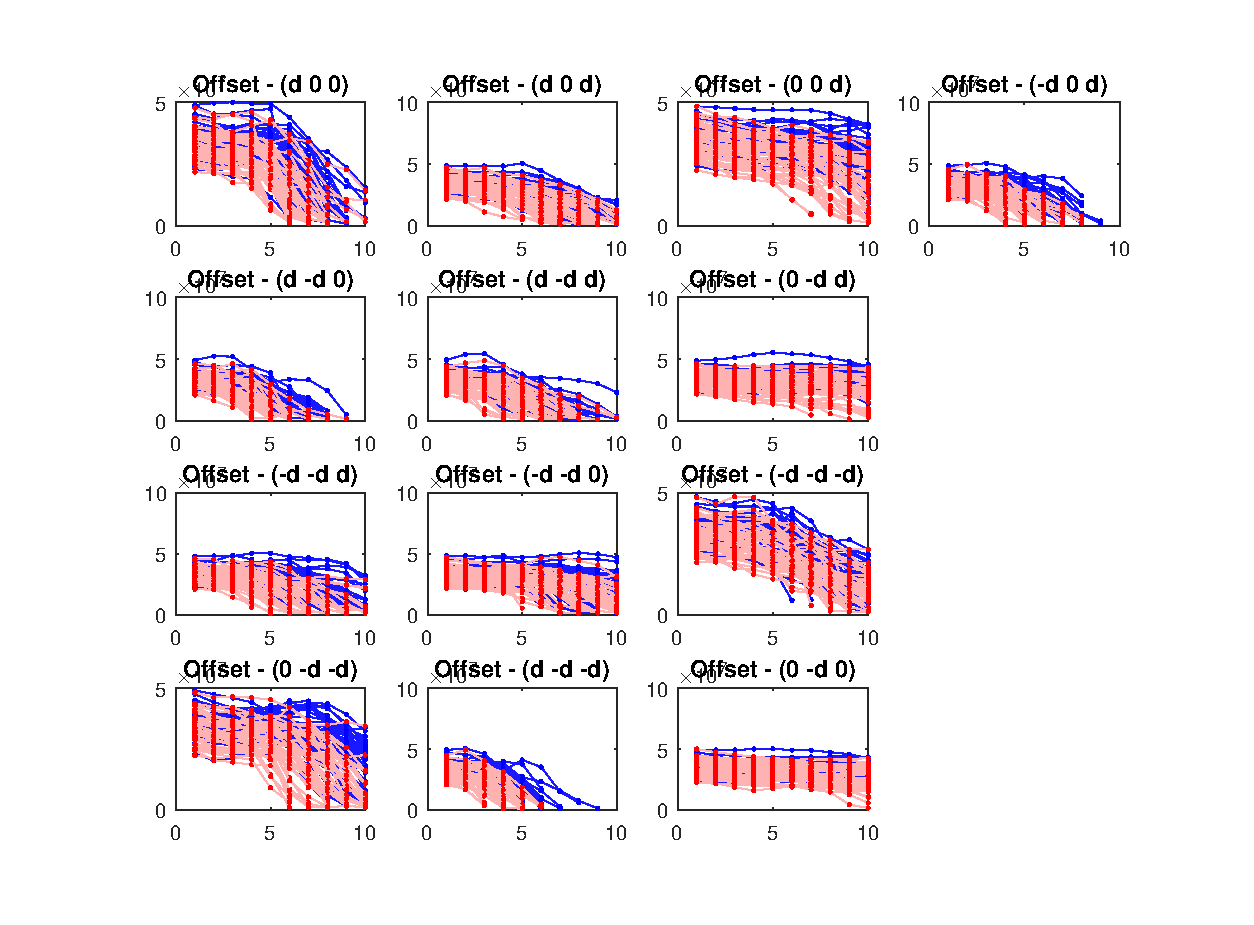
\includegraphics[scale=0.65]{Correlationleftnormalizederode3D.eps}
  \caption{Plot of the Correlation features where the data have been normalized and eroded. The red are the patients with AD and the blue are the rest}\label{fig:Correlationleftnormalizederode3D}
\end{figure}

\begin{figure}[H]
  \centering
  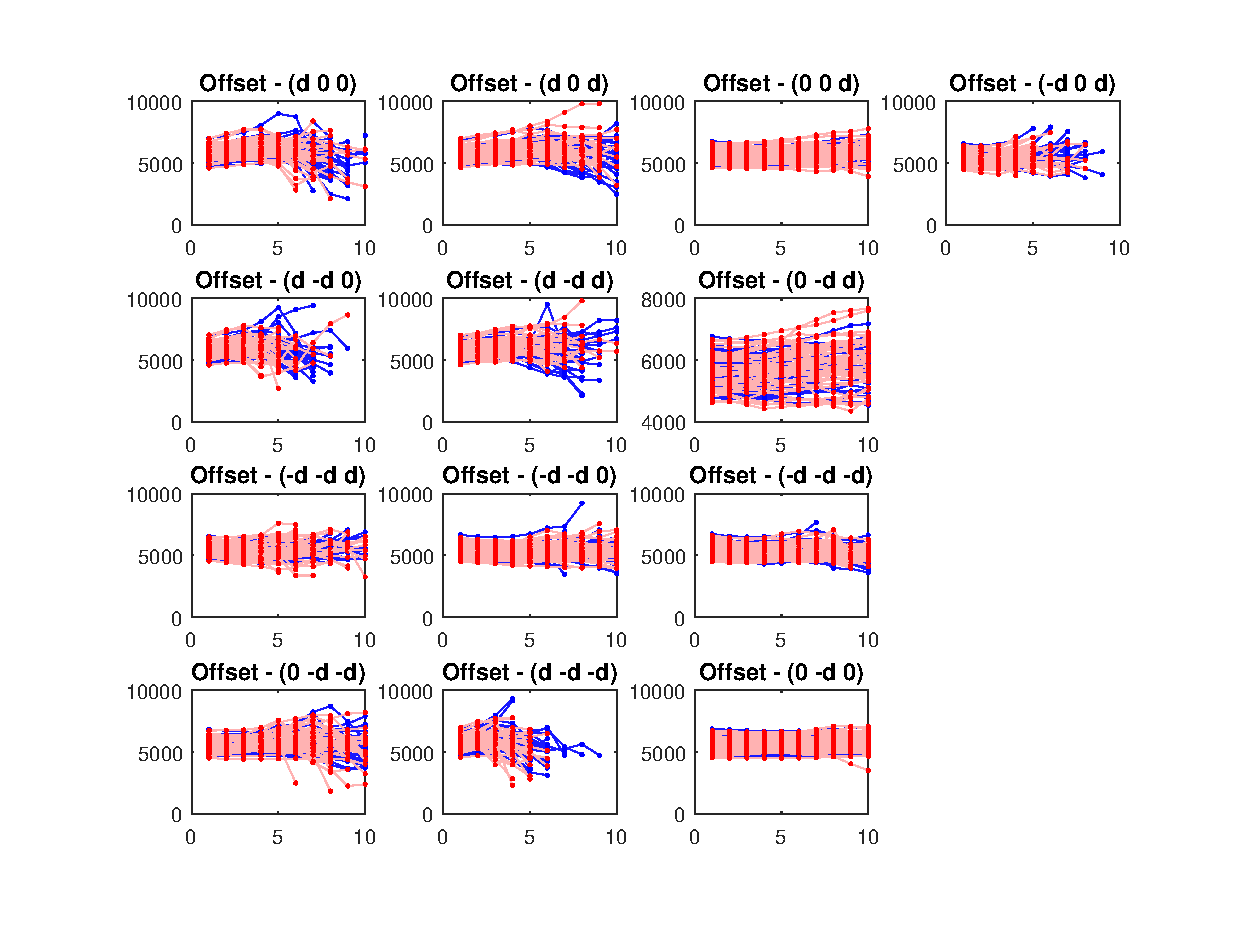
\includegraphics[scale=0.65]{Varianceleftnormalizederode3D.eps}
  \caption{Plot of the Variance features where the data have been normalized and eroded. The red are the patients with AD and the blue are the rest}\label{fig:Varianceleftnormalizederode3D}
\end{figure}

\begin{figure}[H]
  \centering
  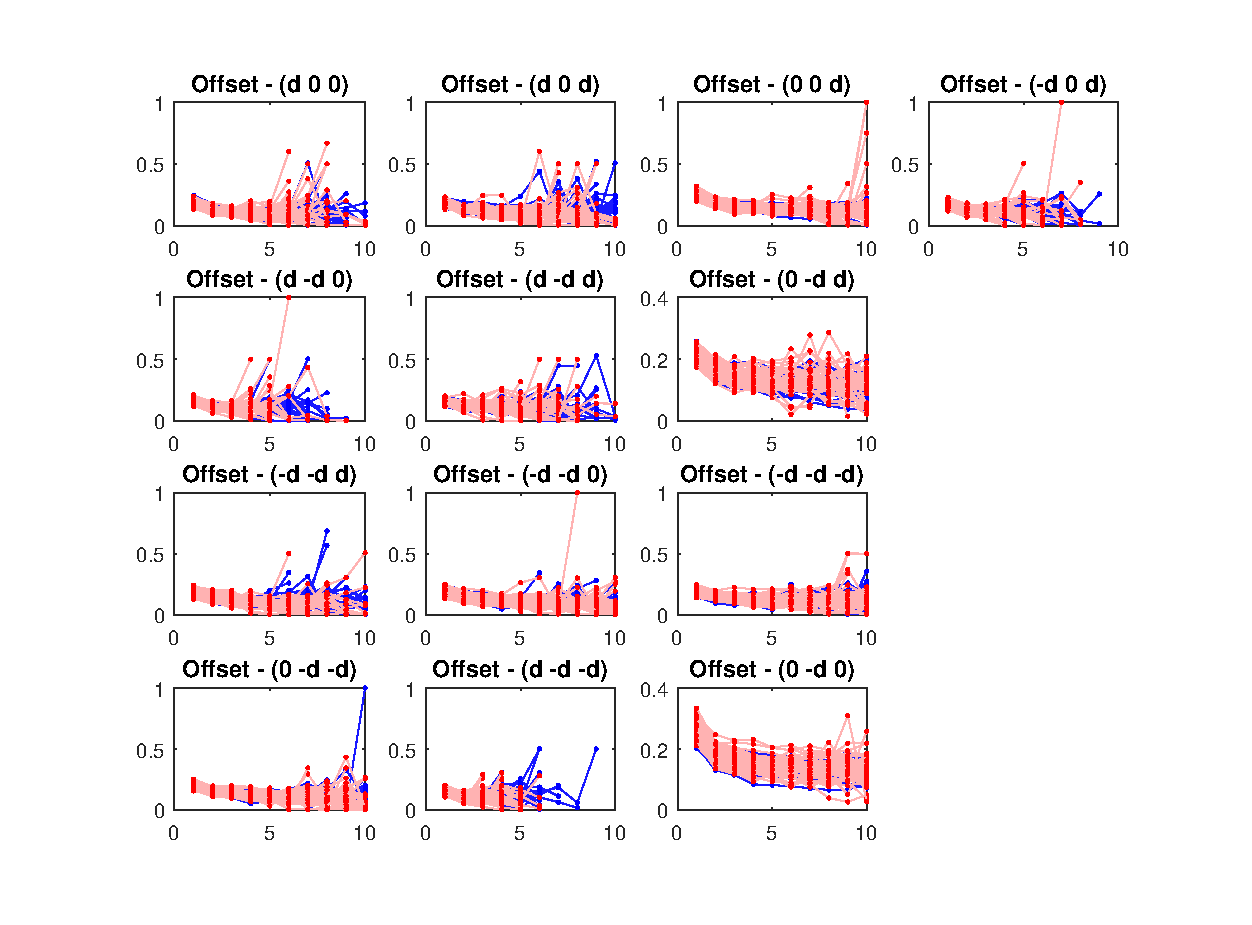
\includegraphics[scale=0.65]{IDMleftnormalizederode3D.eps}
  \caption{Plot of the Inverse Difference Moment features where the data have been normalized and eroded. The red are the patients with AD and the blue are the rest}\label{fig:IDMleftnormalizederode3D}
\end{figure}

\begin{figure}[H]
  \centering
  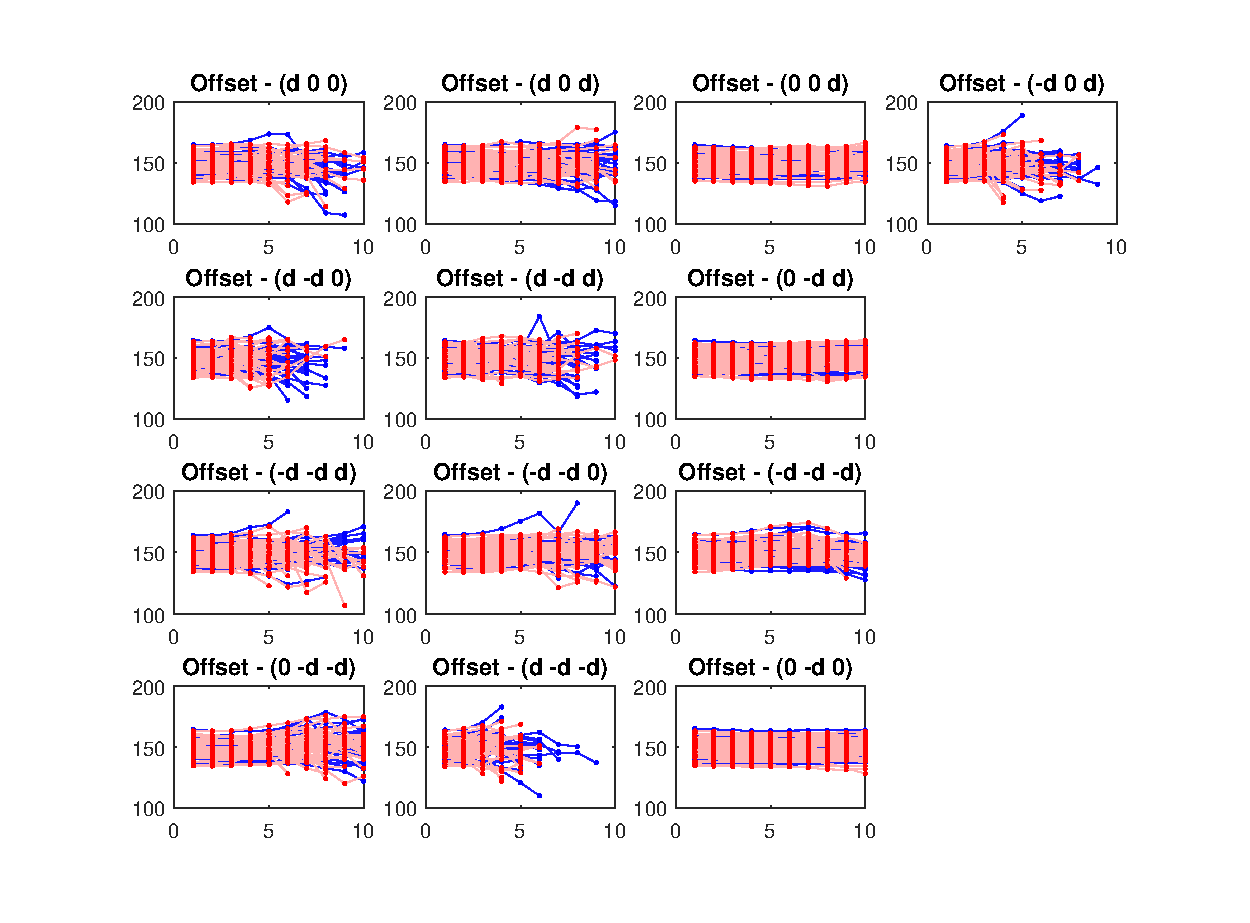
\includegraphics[scale=0.65]{SumAverageleftnormalizederode3D.eps}
  \caption{Plot of the Sum Average features where the data have been normalized and eroded. The red are the patients with AD and the blue are the rest}\label{fig:SumAverageleftnormalizederode3D}
\end{figure}

\begin{figure}[H]
  \centering
  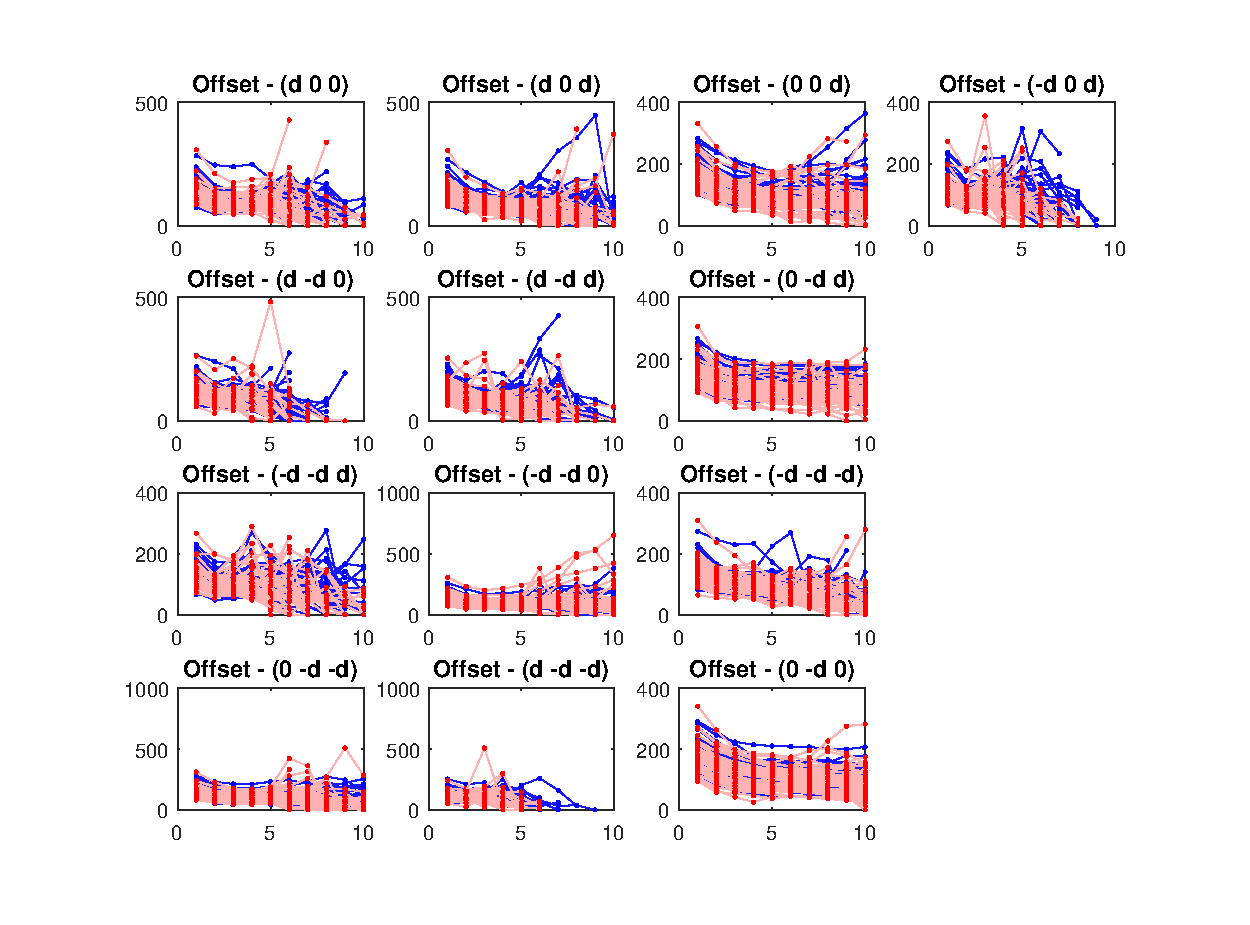
\includegraphics[scale=0.65]{SumVarianceleftnormalizederode3D.eps}
  \caption{Plot of the Sum Variance features where the data have been normalized and eroded. The red are the patients with AD and the blue are the rest}\label{fig:SumVarianceleftnormalizederode3D}
\end{figure}

\begin{figure}[H]
  \centering
  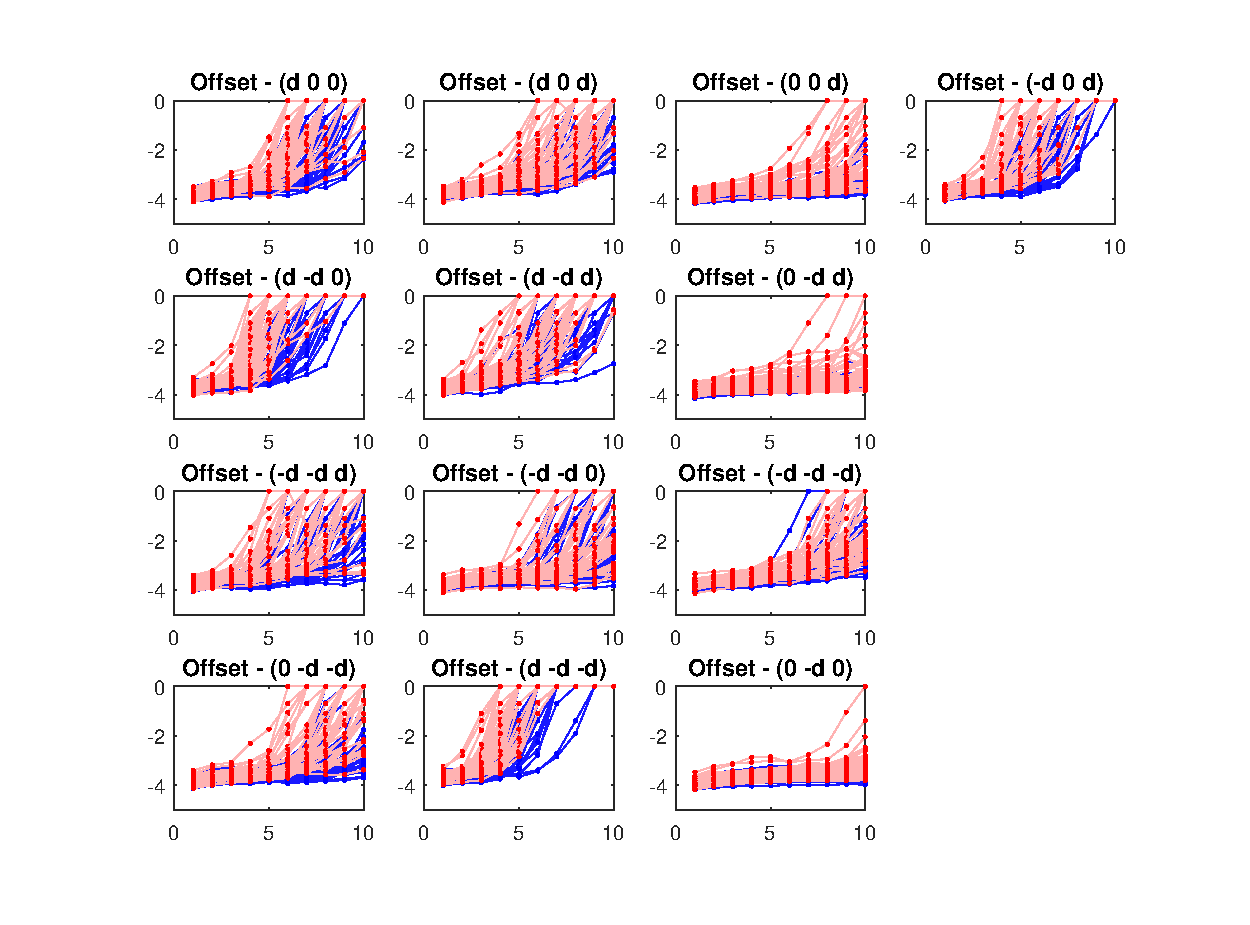
\includegraphics[scale=0.65]{SumEntropyleftnormalizederode3D.eps}
  \caption{Plot of the Sum Entropy features where the data have been normalized and eroded. The red are the patients with AD and the blue are the rest}\label{fig:SumEntropyleftnormalizederode3D}
\end{figure}

\begin{figure}[H]
  \centering
  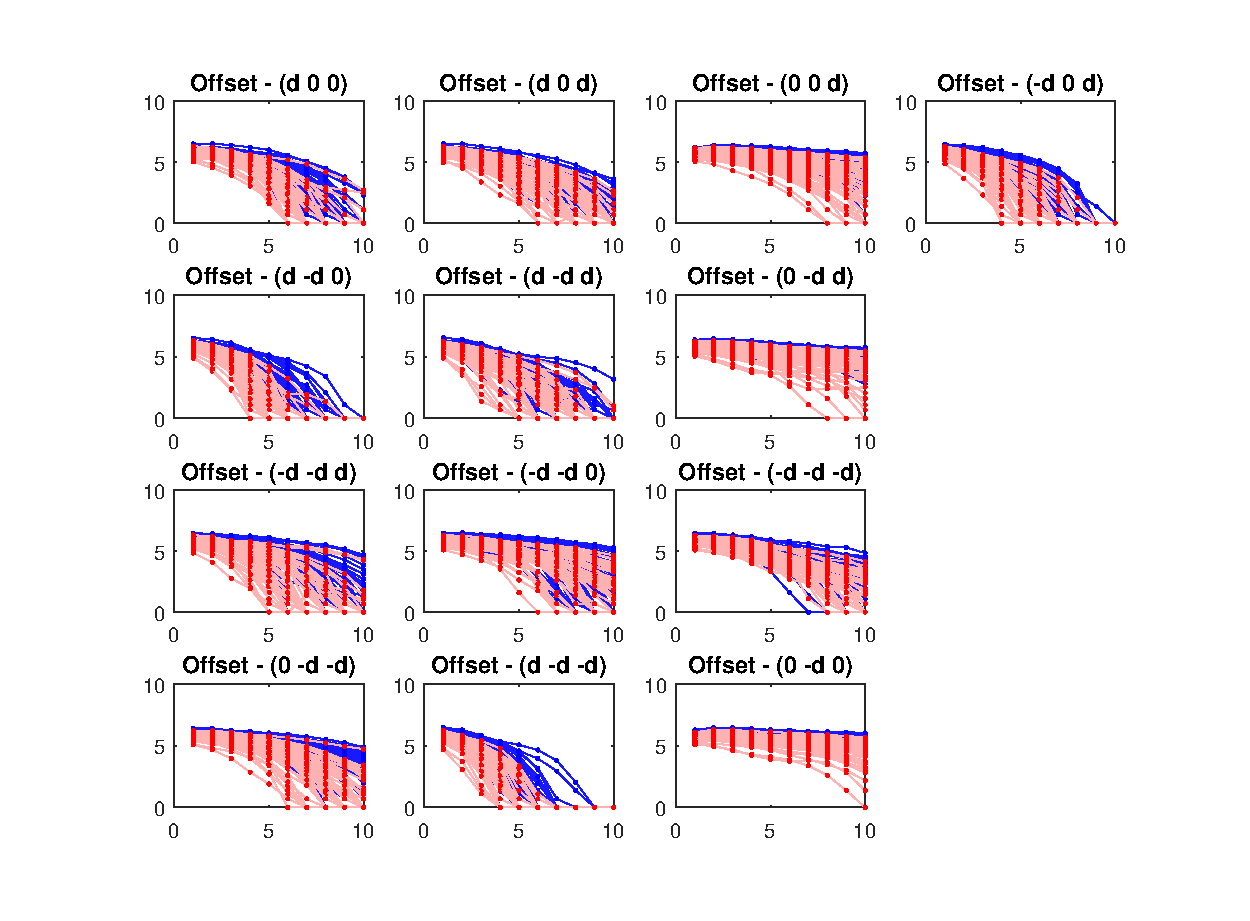
\includegraphics[scale=0.65]{Entropyleftnormalizederode3D.eps}
  \caption{Plot of the Entropy features where the data have been normalized and eroded. The red are the patients with AD and the blue are the rest}\label{fig:Entropyleftnormalizederode3D}
\end{figure}

\begin{figure}[H]
  \centering
  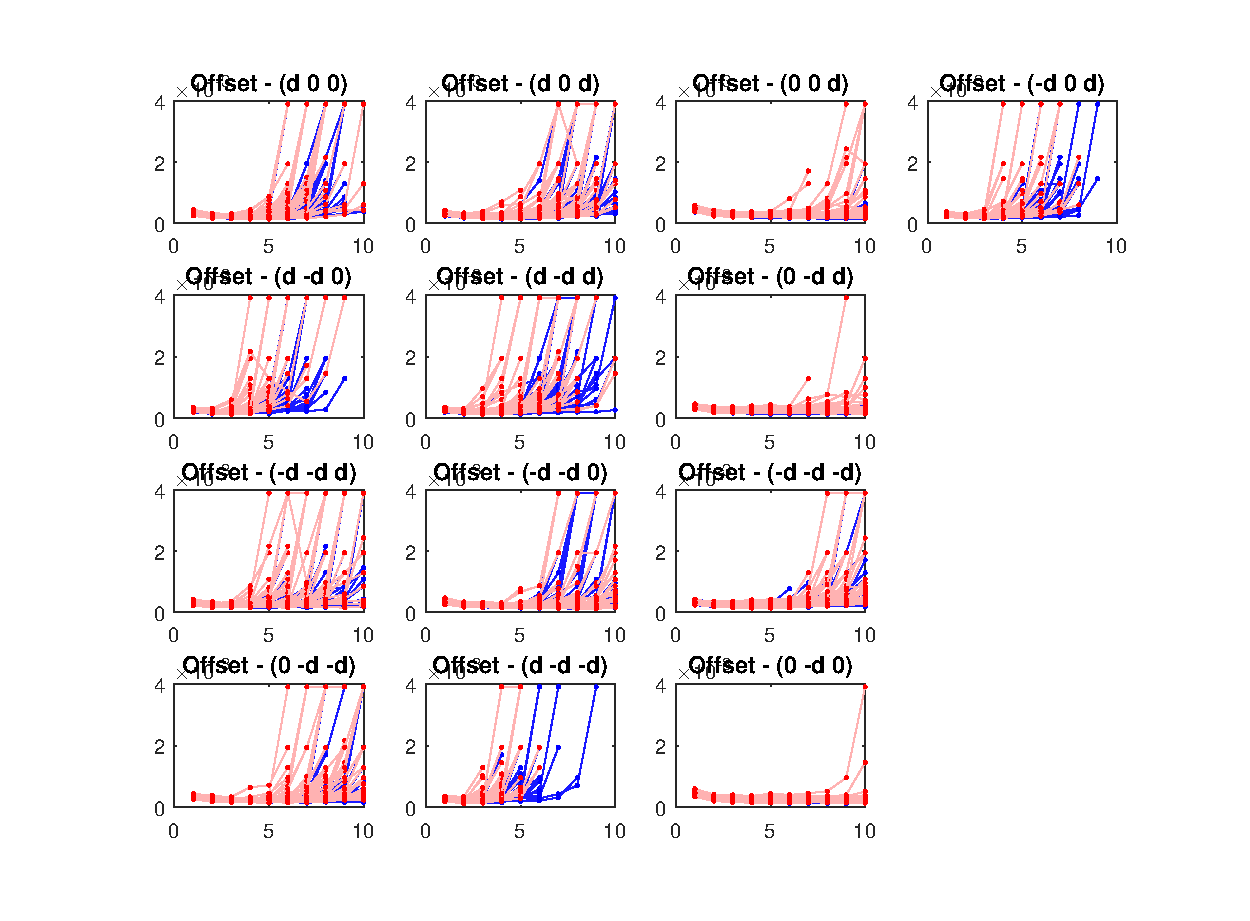
\includegraphics[scale=0.65]{DifferenceVarianceleftnormalizederode3D.eps}
  \caption{Plot of the Difference Variance features where the data have been normalized and eroded. The red are the patients with AD and the blue are the rest}\label{fig:DifferenceVarianceleftnormalizederode3D}
\end{figure}

\begin{figure}[H]
  \centering
  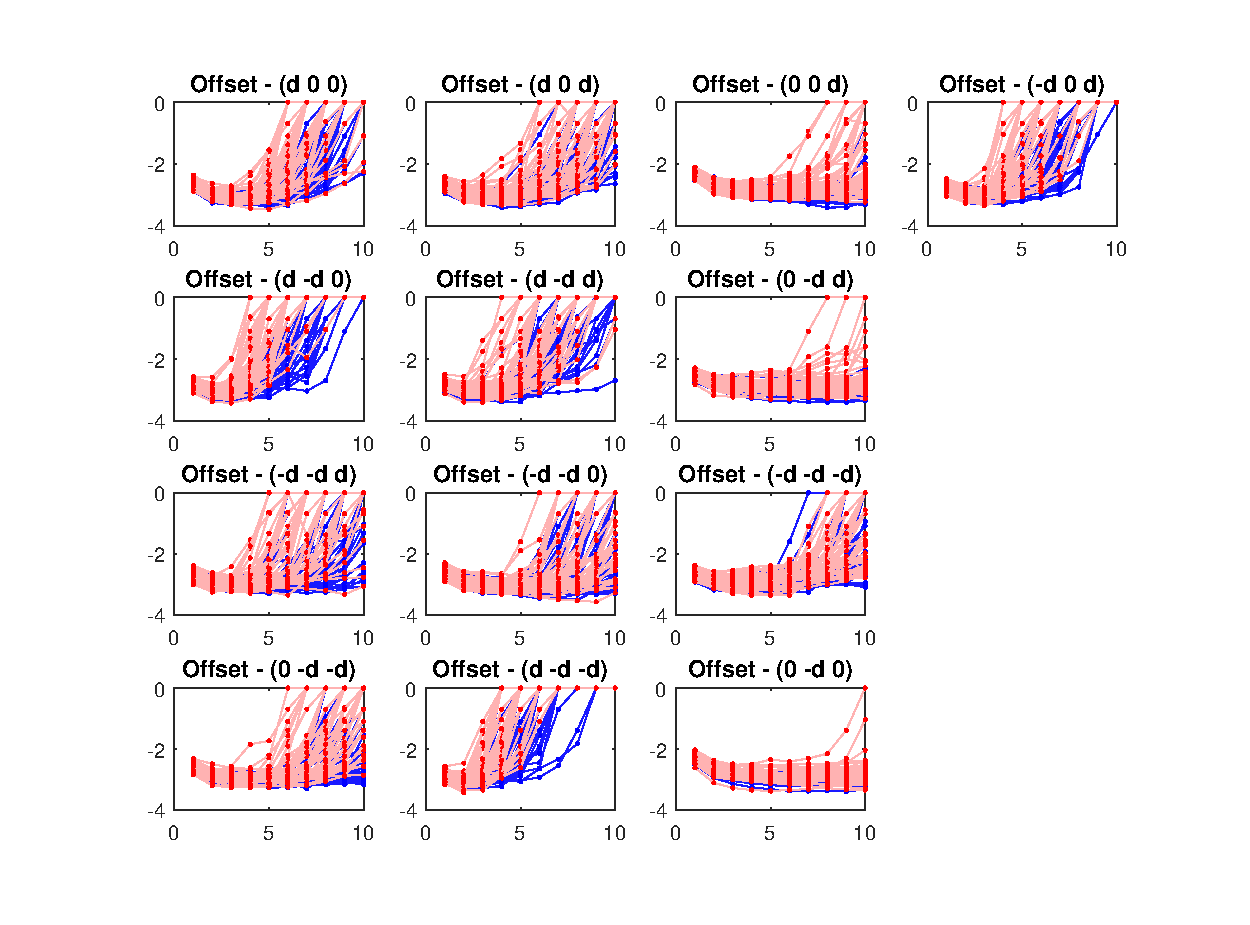
\includegraphics[scale=0.65]{DifferenceEntropyleftnormalizederode3D.eps}
  \caption{Plot of the Difference Entropy features where the data have been normalized and eroded. The red are the patients with AD and the blue are the rest}\label{fig:DifferenceEntropyleftnormalizederode3D}
\end{figure}

\begin{figure}[H]
  \centering
  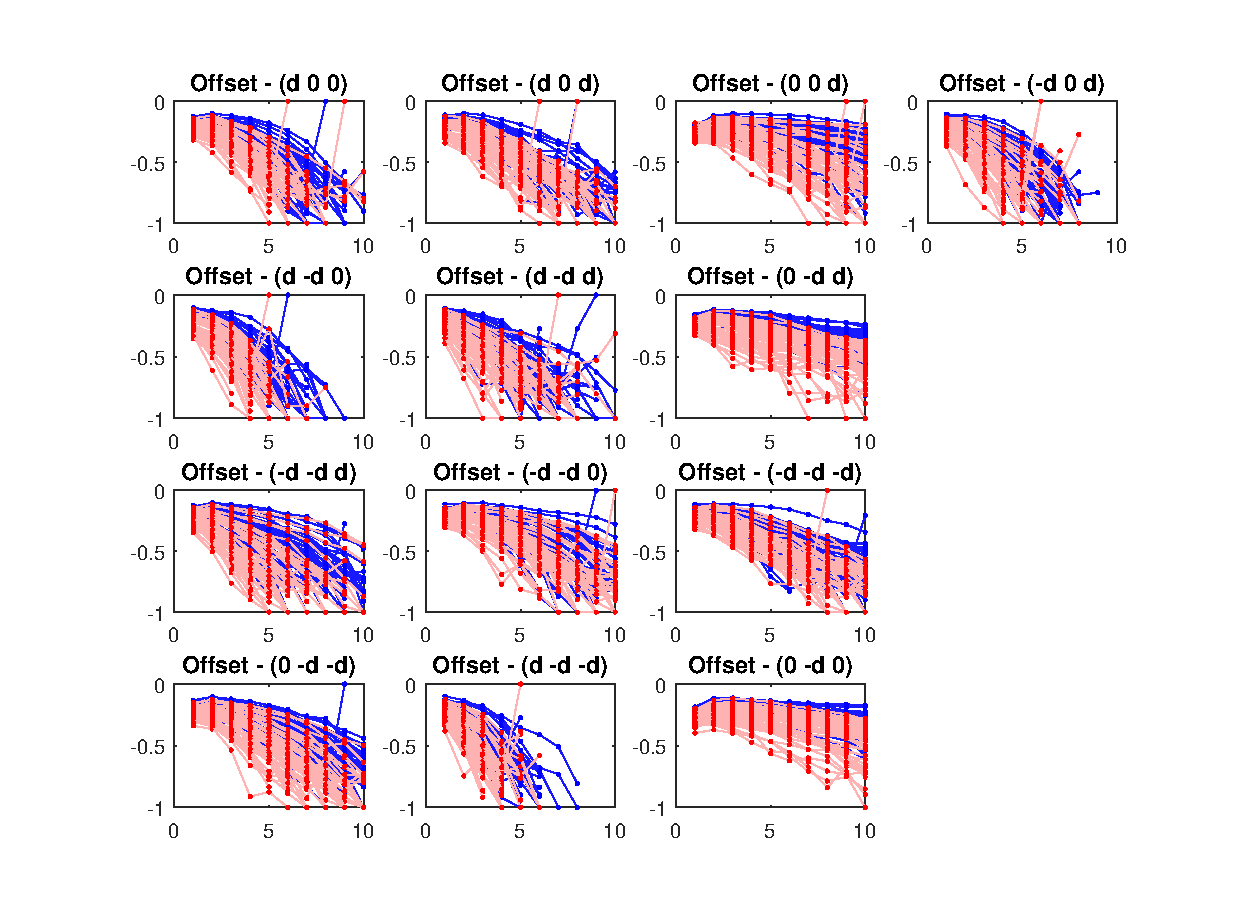
\includegraphics[scale=0.65]{IMOC1leftnormalizederode3D.eps}
  \caption{Plot of the Information Measures of Correlation1 features where the data have been normalized and eroded. The red are the patients with AD and the blue are the rest}\label{fig:IMOC1leftnormalizederode3D}
\end{figure}

\begin{figure}[H]
  \centering
  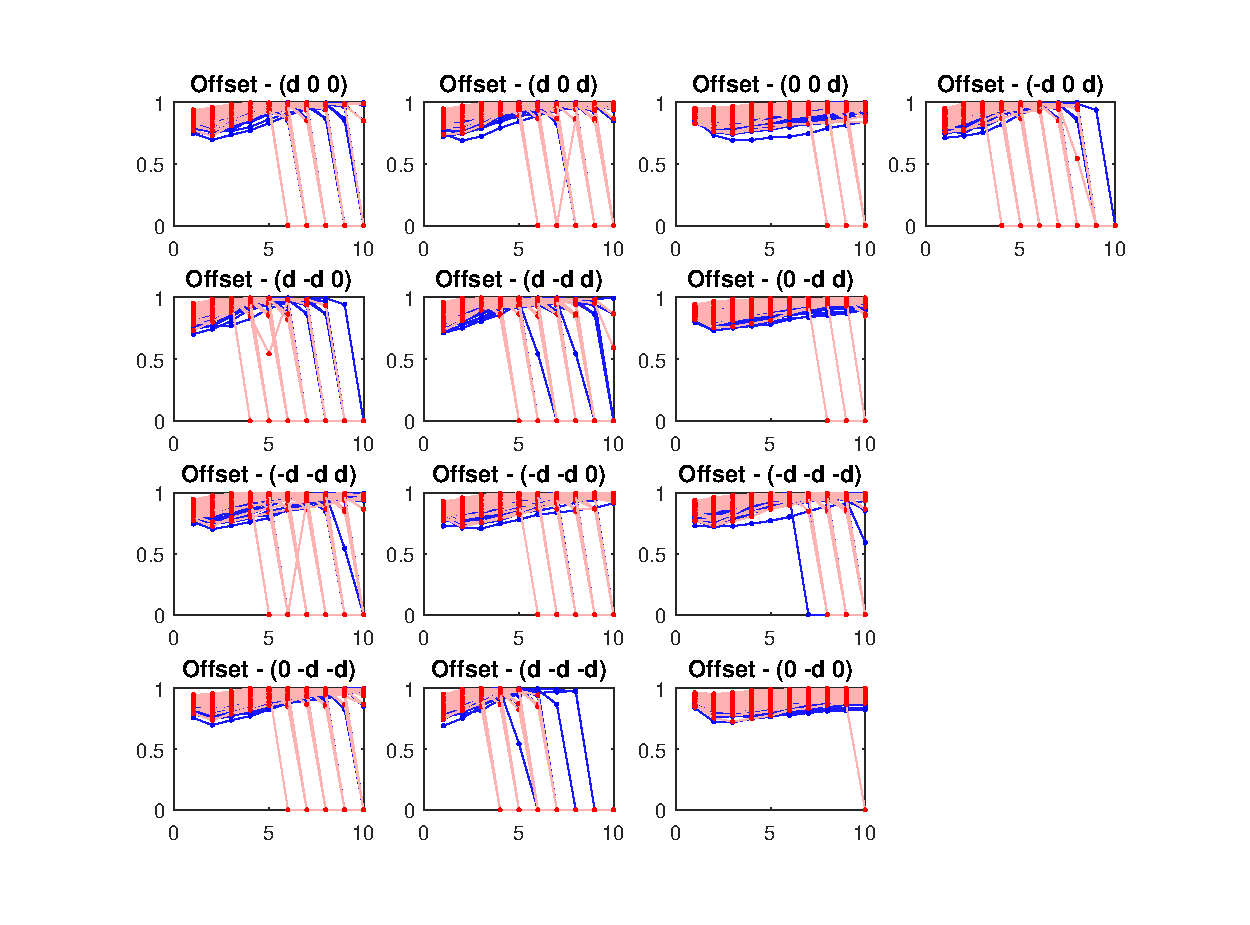
\includegraphics[scale=0.65]{IMOC2leftnormalizederode3D.eps}
  \caption{Plot of the Information Measures of Correlation2 features where the data have been normalized and eroded. The red are the patients with AD and the blue are the rest}\label{fig:IMOC2leftnormalizederode3D}
\end{figure}
